\documentclass[10pt]{report}

\usepackage[headings]{fullpage}
\usepackage{scribe}

% Packages
\usepackage{amsfonts}
\usepackage{amsmath}
\usepackage{amsthm}
\usepackage[letterpaper,margin=1in]{geometry}
 \usepackage{epsfig}
%% \usepackage{color}
%% \usepackage{array}
%% \usepackage{pstricks}
%% \usepackage{pst-plot}
%\usepackage{pstricks-add}

\theoremstyle{plain}
\newtheorem{lemma}{Lemma}
\newtheorem{claim}[lemma]{Claim}
\newtheorem{theorem}[lemma]{Theorem}
\newtheorem{corollary}[lemma]{Corollary}
\newtheorem{prop}[lemma]{Property}

\theoremstyle{definition}
\newtheorem{define}[lemma]{Definition}
\newtheorem{example}[lemma]{Example}

\newtheorem{problem}{Problem}

\newcommand{\E}{\mathbb{E}}
\newcommand{\R}{\mathbb{R}}
\newcommand{\bP}{\mathbb{P}}
\newcommand{\var}{\mbox{\rm var}}
\newcommand{\pr}{\mbox{\rm Pr}}

\def\X{{\cal X}}
\def\Y{{\cal Y}}
\def\cost{{\mbox{\rm cost}}}

\begin{document}

\course{DSE 210}
\coursetitle{Probability and statistics}
\semester{Winter 2015}
\lecturer{}
\scribe{}
\lecturenumber{8}
\lecturetopic{Matrix factorization}

\maketitle

\begin{enumerate}

\item Is the following set of vectors an orthonormal basis of $\R^3$? Explain why or why not.
$$\begin{pmatrix} 3 \\ 4 \\ 0 \end{pmatrix}, \begin{pmatrix} 4 \\ -3 \\ 0 \end{pmatrix}, \begin{pmatrix} 0 \\ 0 \\ 1 \end{pmatrix}$$

\item The following four figures show different 2-dimensional data sets. In each case, make a rough sketch of an ellipsoidal contour of the covariance matrix and indicate the directions of the first and second eigenvectors (mark which is which).

\begin{center}
\begin{tabular}{cc}
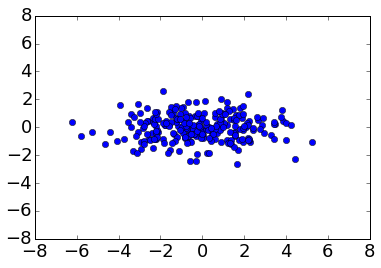
\includegraphics[width=3in]{data1.png}
&
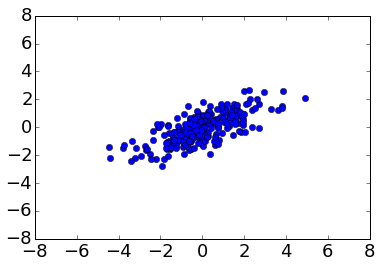
\includegraphics[width=3in]{data2.png}
\\
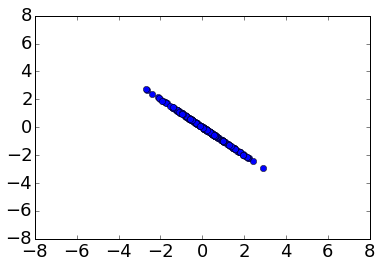
\includegraphics[width=3in]{data3.png}
&
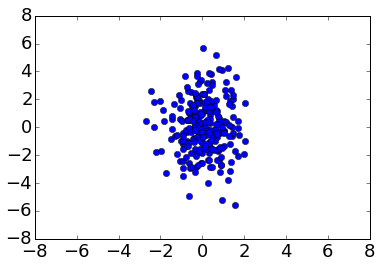
\includegraphics[width=3in]{data4.png}
\end{tabular}
\end{center}

\item Let $u_1, u_2 \in \R^p$ be two vectors with $\|u_1\| = \|u_2\| = 1$ and $u_1 \cdot u_2 = 0$. Define
$$ U = \begin{pmatrix}
\big\uparrow & \big\uparrow \\
u_1          & u_2 \\
\big\downarrow & \big\downarrow
\end{pmatrix} $$
\begin{enumerate}
\item What are the dimensions of each of the following?
\begin{itemize}
\item $U$
\item $U^T$
\item $UU^T$
\item $u_1u_1^T$
\end{itemize}
\item What are the differences, if any, between the following four projections?
\begin{itemize}
\item $x \mapsto (u_1 \cdot x, u_2 \cdot x)$
\item $x \mapsto (u_1 \cdot x) u_1 + (u_2 \cdot x) u_2$
\item $x \mapsto U^T x$
\item $x \mapsto UU^T x$
\end{itemize}
\end{enumerate}

\item Recall the {\it animals with attributes} data set from Worksheet 7, which has information about 50 animals, each represented as a vector in $\R^{85}$.

We would like to visualize these animals in 2-d. Show how to do this with a PCA projection from $\R^{85}$ to $\R^2$. Show the position of each animal, and label them with their names. (Remember from Worksheet 7 how to enlarge the figure. This time you might want to ask for size 10,10.)

Does this {\it embedding} seem sensible to you?

\item In lecture, we looked at the effect of projecting the MNIST data set of handwritten digits to lower-dimension: from 784 to 200, 150, 100, 50 dimensions. We found that the reconstruction error was fairly low for 150-dimensional projections, but noticeable for 50-dimensional projections.

We now investigate these issues further.
\begin{enumerate}
\item Let $X \in \R^p$ have covariance matrix $\Sigma$. Suppose the eigenvalues of $\Sigma$ are $\lambda_1 \geq \lambda_2 \geq \cdots \geq \lambda_p$, and suppose the corresponding eigenvectors are $u_1, u_2, \ldots, u_p$. Then it can be shown that $X$ has an overall variance of $\lambda_1 + \cdots + \lambda_p$, and that when $X$ is projected onto the top $k$ eigenvectors, the residual variance (the information that gets lost) is $\lambda_{k+1} + \cdots + \lambda_p$. Therefore, for this projection, the fraction of lost information, intuitively speaking, is
  $$ F(k) = \frac{\lambda_{k+1} + \cdots + \lambda_p}{\lambda_1 + \cdots + \lambda_p} $$

Compute these fractions for the MNIST data set, for $k = 200, 150, 100, 50, 25$.

\item Suppose we are allowed a different projection for each digit. We would then expect that we can project to an even lower dimension while maintaining roughly the same amount of information. Test whether this is true as follows: for each digit $j = 0, 1, 2, \ldots, 9$,
\begin{itemize}
\item Obtain the PCA projection to $k$ dimensions, for $k = 200, 150, 100, 50, 25$.
\item Compute the fraction $F_j(k)$, for each such value of $k$.
\item Pick a random instance of the digit. Show the original digit as well as its reconstruction at each of these five values of $k$. (Note: the original images have pixel values in the range 0-255, but this might not be true of the reconstructions; therefore, you may need to clip the reconstructed pixels to lie within this range before displaying the image.)
\end{itemize}
Show all the fractions $F_j(k)$ in a table. Which digit seems to be the most amenable to low-dimensional projection?
\end{enumerate}

\end{enumerate}

\end{document}
\item A police station wishes to collect statistics on incoming calls. A particular work week is partitioned into $5 \times 8 \times 6 = 240$ intervals of 10 minutes each, and the number of calls received during each interval is noted. Let $N_k$ denote the number of intervals in which $k$ calls were received. The following data was obtained:
\begin{tabular}

\end{tabular}
 
